\vspace{10ex}
\chapter{Impact}
\label{cha:impact}

\section{Expected impacts} 
\label{sec:expected-impact}


We will empower even small companies to offload the costs of their internal IT,
and gain technological independence over their connected computing resources.
\textit{iWe} is basically identifying and fixing gaps in cloud efficiency that
SMEs can't currently avoid.  In this section we will briefly describe our Total
cost of ownership (TCO) analysis, our powerful internal IT architecture, the
potential we have to save up to 50\% in power consumption, and how we plan to
further reduce costs for our customers designing, building, and selling our own
cloud hardware.

\subsection{Internal IT powered by \textit{iWe}} 
\label{subsec:iitic}

In the past the minimum possible setup for a reliable and flexible internal IT
would include two servers for redundancy and a storage device that also offers
redundancy. The need of a storage device adds complexity, increase acquisition
costs and complicates maintenance.  The storage is needed to physically separate
data from servers, allowing a key technical feature named \textit{live
migration}.

\textit{Live migration} is a feature that allows to move virtual machines, and
other resources, between different physical servers, \textbf{while the resources
are running}, and without noticeable interruption. It is extremely valuable for
maintenance and for fault tolerance, and the lack of \textit{live migration} is
not acceptable.

Using the \textit{iWe} server architecture the minimum possible setup uses
only two servers, and there is no need for a dedicated storage device. Instead
of physically separating data from servers, instead of using an external and
shared storage device, we keep the data synchronized on multiple servers, saving
one copy of the data on each server.  This design allows for \textit{live
migration} at a fraction of complexity and costs. While this is not the best
configuration for large scenarios, it is clearly more efficient for environments
with small server count.

We tested the performance (bandwidth and latency) of our synchronization
technique on SSD disks, and the results were positive. We could reach
native SSD speeds with marginal increase in CPU load, suggesting that our
synchronization mechanism offer performance increase over entry level storage
devices that are popular for SMEs.

The \textit{iWe} server architecture also includes the \textit{iWe}
software stack and \textit{iWe} services. On our side we use highly automated
disaster and attack management which allows us to assume responsibility of
maintenance and support over the Internal IT of our customers. Our customers
save on acquisition, and on expensive system administration skills. As an
example of the efficiency gain provided by the \textit{iWe} server
architecture, our customer can have the double of servers with excellent
savings.

\subsection{TCO for our Internal IT customer} 
\label{subsec:tco}
\begin{table}
    \centering
    \begin{tabular}{r l l | l}
                                    & internal IT     & public cloud      &
                                    SME \textit{iWe Provider}          \\
        \hline
        Full Time engineer          & \SI{225000}[\$]{} & \SI{0}[\$]{}      
                                    & ~\SI{0}[\$]{}      \\
        \hline
        Initial investment          & \SI{123048}[\$]{} & \SI{0}[\$]{}      
                                    & ~\SI{45366}[\$]{}  \\
        \hline
        Services                    & \SI{0}[\$]{}      & \SI{113760}[\$]{} 
                                    & -\SI{28800}[\$]{} \\
        \hline
        Power and Cooling           & \SI{9665}[\$]{}   & \SI{0}[\$]{}      
                                    & ~\SI{6020}[\$]{}   \\
        \hline
        TOTAL                       & \SI{357713}[\$]{} & \SI{113760}[\$]{} 
                                    & ~\SI{22586}[\$]{}  \\
    \end{tabular}
    \caption{3 years TCO showing the SME \textit{iWe Provider} savings}
    \label{table:clouds-comparison}
\end{table}


Total cost of ownership (TCO) is a financial estimate intended to help buyers
and owners determine the direct and indirect costs of a product or system.  We
will compare TCO of traditional internal IT, public cloud services, and of our
SME \textit{iWe Provider}. We use estimations from The Cloud
Calculator \cite{tcc} \footnote{We use US Dollars as currency because The Cloud
Calculator uses US Dollars.} for the traditional IT and public cloud services.
Table \ref{table:clouds-comparison} shows 3 years TCO comparison for a small
cloud infrastructure: 128 GB of RAM, 1000 GB of disk space, with N+1 redundancy. 

The TCO for the first column showing traditional internal IT includes the
acquisition of 2 physical servers, VMWare licenses, Storage Area Network (SAN),
Network Switches, Server Cabinet, and PDUs. It also include costs for Power,
Cooling, and a full time engineer to manage the environment. 3 years TCO:
\SI{357713}[\$]{}. This TCO is a possible scenario for an SME, but is completely
unrealistic for companies such as Google, Amazon, Facebook, and Microsoft, as
they have very efficient resources with impressively low TCO.

We provide the estimated TCO for the SME \textit{iWe Provider}.  The
acquisition costs includes 4 Dell T430 tower servers (\SI{10641}[\$]{}
each) \cite{T430}, UPSs, and Network Switches. It also include costs for Power,
Cooling. However we estimate that our customer will make \SI{28800}[\$]{} with
the surplus of server capacity, and as the skills the \textit{iWe Provider}
needs to manage the environment is of a \textbf{power user} there are no
expenses with a full time engineer. 3 years TCO: \SI{22586}[\$]{}. We made our
estimations based on a \textit{Cloud unit} that link computational resources and
equivalent monthly value:

\begin{equation}
    1 Cloud_{unit} = 1 CPU_{core} + 2 GB_{ram} + 20 GB_{ssd} \equiv \SI{20}[\$]{}/month
\end{equation}

The physical servers of our solution are configured to provide multiples of the
\textit{Cloud unit} in at least N+1 redundancy. N+1 redundancy reduces by half
the amount of RAM memory and disk space that are usable. After the redundancy
losses, the four servers of the Internal IT powered by \textit{iWe} from
Table \ref{table:clouds-comparison} and shown on Figure
\ref{fig:the-clalld-pvt-pub} provide:

\begin{equation}
    160 Cloud_{units} = 160 CPU_{core} + 320 GB_{ram} + 3200 GB_{ssd} \equiv
    \SI{3200}[\$]{}/month
\end{equation}

Which gives 80 \textit{Cloud units} for private use, and 80 \textit{Cloud units}
for offloading costs, including the \textit{iWe} services. The share of
resources we are going to take in exchange of our private cloud services is to
be defined, but we used \textbf{20\%} in our examples.

\begin{equation}
    iWe_{share} = 160 Cloud_{units} * 20\% = 32 Cloud_{units} * 36 months
    \equiv \SI{23040}[\$]{}
\end{equation}

Taking 32 \textit{Cloud units} for covering the \textit{iWe} costs leaves the
customer with \textbf{48 \textit{Cloud units}} for cost offloading. To avoid
over optimistic estimations we used approximately 80\% of the 48 \textit{Cloud
units} resulting:


\begin{equation}
    Customer_{offloading} = 40 Cloud_{units} * 36 months \equiv \SI{28800}[\$]{}
\end{equation}

Which takes us to the \textit{iWe} solution being 15 times cheaper than
traditional IT:

\begin{equation}
    \frac{internal~IT_{TCO}}{powered~by~iWe_{TCO}} =
    \frac{\SI{357713}[\$]{}}{\SI{22586}[\$]{}} =
    15.83
\end{equation}

\subsection{\textit{iWe} Hardware} 
\label{subsec:ch}

\begin{figure}
    \centering
    \begin{minipage}{0.5\textwidth}
        \centering
        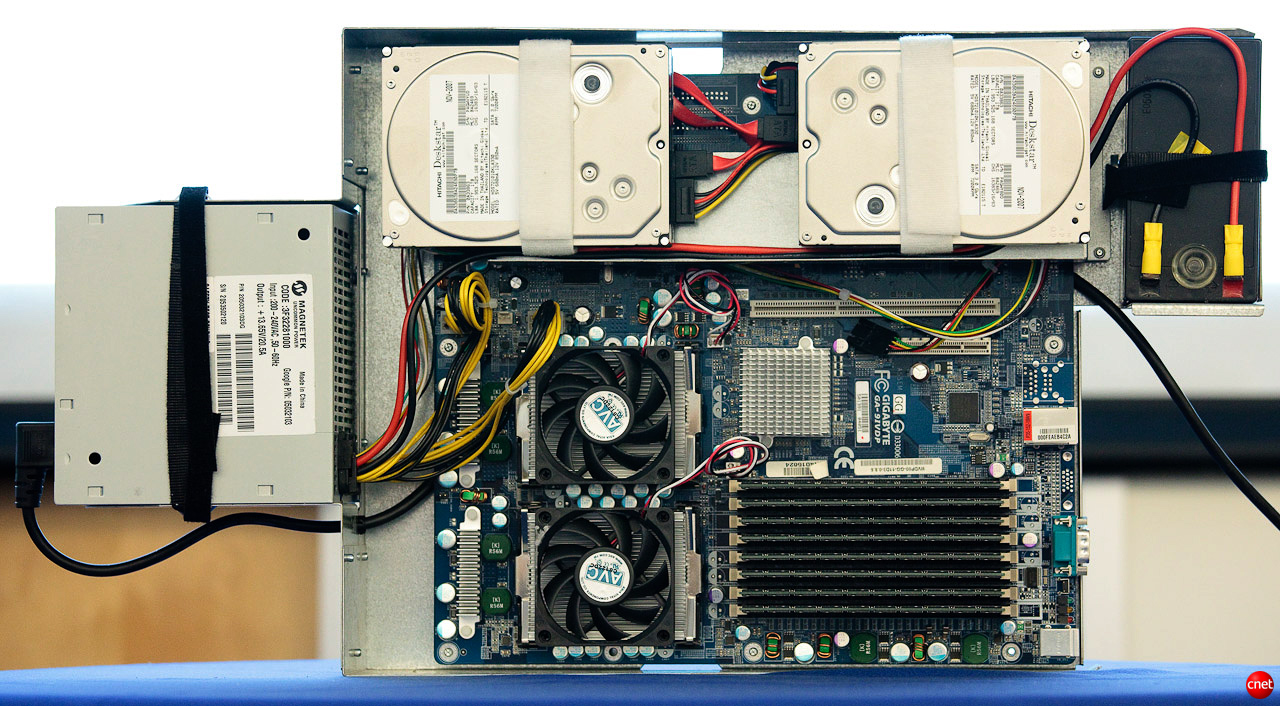
\includegraphics[width=0.83\textwidth]{images/GoogleServerLarge}
        \caption{First generation of custom Google server}
        \label{fig:google1stsrv}
    \end{minipage}%
    \begin{minipage}{0.5\textwidth}
        \centering
        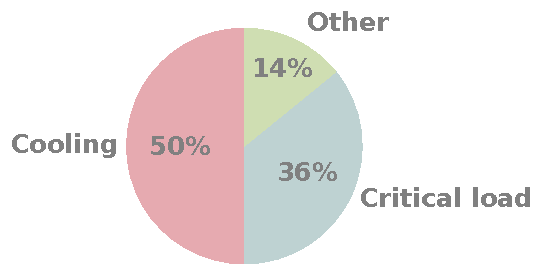
\includegraphics[width=0.9\textwidth]{images/power-pie.pdf}
        \caption{Data center power consumption}
        \label{fig:power-bd}
    \end{minipage}%
\end{figure}

We can offer great savings even when using stock, high-end, and expensive
servers such as the Dell T430 \cite{T430} that we use in our example. The problem
is that using stock servers is very expensive. Exactly as the TCO of the
traditional internal IT of Table \ref{table:clouds-comparison} is unrealistic
for companies such as Google and Amazon, the price of \SI{10641}[\$]{} for the
resources provided by our Dell T430 is also unrealistic for them. Google,
Amazon, and Facebook design and build their own hardware with total focus on
efficiency.

Google uses custom built servers for more than 10 years now, Figure
\ref{fig:google1stsrv} \cite{cnetgsrv} shows a Google server from 2006. Every
component of the Google server is there to minimize the TCO, including the open
case, and the battery. Following the efficiency masters, we will design, build,
and sell our own high-end low cost hardware, which will be the next step in
reducing costs of connected computing resources for our customers, helping them
to be more competitive.

\subsection{Electrical Efficiency} 
\label{subsec:ee}

% Describe how your innovation will contribute to any substantial impact
% addressing issues related to climate change or the environment, or bring other
% important benefits to society.

The \textit{iWe} decentralized architecture doesn't require the equipment
density of a typical data center, which is an opportunity to reduce power
consumption with cooling. In a typical data center only 36\% of power is used
for the critical load such as servers and networking equipment, cooling alone
consume 50\%, and the remaining 14\% are consumed by other important loads
\cite{apc-dc-power}.  Figure \ref{fig:power-bd} illustrates a breakdown of how
electricity is consumed among the various loads in a typical data center
\cite{apc-dc-power}. The lower server density of \textit{iWe} architecture is
an opportunity to save up to 50\% in power consumption, which has very positive
environmental impact.

If we opted for the typical data center approach for our small scale deployment,
we would install all our notebooks in a single location, which would require
using a small air conditioning unit. This air conditioning unit would at least
match the power consumption of our notebooks\footnote{All power that is consumed
by IT equipment is converted to heat. Though power is typically reported in
watts (W) and heat is typically reported in British Thermal Units (BTUs), these
units are in fact interchangeable \cite{cisco-dc-power}.}, multiplying by two
the total power consumption of our small scale deployment. However we are going
to use our distributed architecture, and we will install our notebooks in 20
different locations, which will not require the addition of per-location cooling
systems.  Our architecture allows us to save 50\% in power consumption compared
to the typical data center approach.

\subsection{Commercial Potential}
\label{subsec:company}

% How does the innovation project fit with the strategy of the participating
% SME(s)

% What is the relevance and rationale of the innovation project for the
% management team of the SME (or lead SME(s) in a consortium)

% What is the expected growth potential of your solution in terms of turnover,
% employment, market seize, IP management, sales, return on investment and
% profit etc.

While the SME \textit{iWe Provider} of our example get cloud resources 15
times cheaper, we make \SI{23040}[\$]{} in 3 years with the provision of our
services.  There is a long road ahead of us before our services are ready for
the market, but our business model and cloud architecture suggest that we will
offer an exceptional service with low operational costs. We have to carefully
define metrics before making reasonable financial estimations, but we can make
an educated guess based on our example SME \textit{iWe Provider}.  This
customer gives us \SI{640}[\$]{} per month, but we can make an estimation based
on 33\% of that value. If we make \SI{214}[\$]{} per month per \textit{iWe
Provider}, we can reach a monthly turnover of \SI{1}[\$]{M} with less than 5000
customers:

\begin{equation}
    \SI{1}[\$]{M}_{turnover} = \frac{\SI{1000000}[\$]{}}{\SI{214}[\$]{}} = 4673~Customers
\end{equation}

We believe it is feasible to have 5000 small \textit{iWe Providers} in our
first year of operation. 5000 customers is 0.005\% of the estimated 1M public
cloud customers Amazon had in the end of 2015 \cite{howlongaws}. And we expect
to be able to handle the first 5000 \textit{iWe Provider} customers with a
team of approximately 25 employees. We also expect that the number of
\textit{iWe Providers} per \textit{iWe} employee will increase with scale,
reducing our expenses per customer.

\section{Measures to maximize impact} 
\label{sec:maximize-impact}
% Explain an initial plan for full commercialisation of the project results,
% i.e. own commercialisation or licensing? Need of cooperation with third
% parties for own commercialisation? Estimate of the total funding requirements?
% Approximate time to first sales/employment?

% How does the proposed work in Phase 1 of the SME instrument fit into the
% overall plan to reach market?

% Outline the status and the strategy for knowledge protection. If by patent,
% has a patent application already been filed or is there potential for patent
% application?

We are working on our business plan, but before we make estimations we need to
collect real world commercial and technical data. However we do know that
commercialization of \textit{iWe} will require development before going to
market, and we expect to need capital to cover our burn rate for up to one year
until we have income.

The known need of investment to cover our pre-income stage makes the the small
scale deployment vital. We will make a small scale deployment to test our
prototype, and to collect real world technical and commercial data that we need
on our business plan.  We are going to deploy our prototype to 10 locations in
Zug to test our solution in a real world scenario.

\textbf{Our small scale deployment test in Zug will provide us with real world
data for supporting our request for capital to cover the pre-income stage of
\textit{iWe}.}
